\documentclass[10pt,a4paper]{article}

\usepackage[margin=0.75in]{geometry}
\usepackage{amsmath,amssymb,amsfonts}
\usepackage{graphicx}
\usepackage{booktabs}
\usepackage{hyperref}
\usepackage{microtype}
\usepackage{caption}
\usepackage{fancyhdr}
\usepackage{titlesec}

% Page setup - Clean Monochrome Academic Journal Styling
\pagestyle{fancy}
\fancyhf{}
\rhead{\small \textit{IEEE Transactions on Computational Imaging} --- Methodological Briefing}
\lhead{\small Single-Photon Computational Imaging \& Machine Vision}
\rfoot{\small Page \thepage\ of 4}
\lfoot{\small IC-PINOT Technical Overview}
\renewcommand{\headrulewidth}{0.4pt}
\renewcommand{\footrulewidth}{0.4pt}

% Section formatting - Formal Academic Styling
\titleformat{\section}{\large\bfseries}{\thesection}{1em}{}[\titlerule]
\titleformat{\subsection}{\normalsize\bfseries}{\thesubsection}{1em}{}

\hypersetup{
    colorlinks=false,
    pdfborder={0 0 0}
}

\begin{document}

% ----------------------------------------------------------------------
% TITLE & HEADER
% ----------------------------------------------------------------------
\begin{center}
    {\LARGE \textbf{IC-PINOT: In-Context Physics-Informed Neural Operator Transformer for Defocus-Invariant Single-Photon Computational Imaging}}\\[4pt]
    {\large \textbf{Industrial Surface Defect Inspection Under Extreme Photon Starvation, Machinery Vibration, and Dynamic Material Changeovers}}\\[6pt]
    \textbf{Open-Source Code \& Checkpoints:} \url{https://github.com/atharveeee-netizen/pi-ghost-transformer}
\end{center}
\vspace{-4pt}
\hrule
\vspace{6pt}

% ----------------------------------------------------------------------
% ABSTRACT & INDEX TERMS (PAGE 1)
% ----------------------------------------------------------------------
\noindent \textbf{\textit{Abstract}}—\textbf{Automated surface defect inspection in high-speed manufacturing faces three simultaneous physical bottlenecks: photon starvation at meter-per-second conveyor velocities, optical defocus induced by mechanical loom vibrations, and catastrophic distribution shifts across dynamic material changeovers. Conventional line-scan cameras require intense lighting, suffer severe motion blur, and lose focus under continuous oscillation. In this work, we eliminate multi-pixel sensors entirely and implement Single-Photon Computational Ghost Imaging (CGI), replacing multi-pixel detector grids with structured light illumination and a single-pixel Single-Photon Avalanche Diode (SPAD). To invert these compressive, photon-starved measurements, we introduce IC-PINOT (In-Context Physics-Informed Neural Operator Transformer). IC-PINOT integrates a continuous Fourier Neural Operator (FNO) that directly encodes optical wave propagation to provide strict invariance to lens defocus up to 3.0 waves ($\Delta\text{PSNR} < 10^{-5}$ dB). An In-Context Prompt Engine enables instant test-time adaptation to unseen materials in 7.2 ms (138 FPS) with zero gradient backpropagation. Furthermore, an evidential Normal-Inverse-Gamma (NIG) parameter head deterministically separates photon shot noise from structural anomaly novelty in a single pass. Across 17 industrial benchmarks, IC-PINOT outperforms classical Differential Ghost Imaging by up to +10.17 dB PSNR and maintains 13.76 dB at extreme 1.0\% sub-Nyquist sampling.}

\vspace{4pt}
\noindent \textbf{\textit{Index Terms}}—\textbf{Computational ghost imaging, Fourier neural operators, single-photon avalanche diodes, in-context learning, evidential uncertainty quantification, defect inspection.}
\vspace{6pt}

% ----------------------------------------------------------------------
% SECTION I: INTRODUCTION (PAGE 1)
% ----------------------------------------------------------------------
\section{Introduction and Industrial Problem Formulation}
In modern industrial textile weaving, automated rapier and air-jet looms operate at continuous line speeds exceeding 1 to 2 meters per second. Microscopic anomalies---including broken yarns, warp knots, thread dropouts, and oil contamination---cause catastrophic loss if continuous fabric rolls are not inspected in real time. However, conventional industrial line-scan and area-scan cameras face three fundamental physical bottlenecks:
\begin{enumerate}
    \setlength\itemsep{-2pt}
    \item \textbf{Photon Starvation and Motion Blur:} Operating at meter-per-second velocities restricts optical exposure times to microseconds. Under low ambient photon flux, individual camera pixels receive insufficient signal, resulting in images dominated by thermal and electronic readout noise.
    \item \textbf{Machinery Vibration Defocus:} Industrial weaving machinery generates continuous mechanical oscillation. This oscillation continuously modulates the physical distance between the imaging objective and the moving fabric, inducing time-varying optical defocus that severely blurs fine defect boundaries.
    \item \textbf{Dynamic Material Variations:} Commercial weaving plants alternate fabric weaves (cotton, twill, denim, silk, and technical synthetics) on a daily basis. Standard supervised convolutional neural networks degrade severely when evaluated on textile weaves outside their narrow training distribution.
\end{enumerate}

% ----------------------------------------------------------------------
% SECTION II: PHYSICAL PRINCIPLES (PAGE 1)
% ----------------------------------------------------------------------
\section{Physical Principles of Computational Ghost Imaging}
Single-Photon Computational Ghost Imaging (CGI) resolves these constraints by decoupling spatial resolution from the optical detector. Rather than relying on a multi-pixel focal plane array, the physical system operates as follows:
\begin{enumerate}
    \setlength\itemsep{-2pt}
    \item \textbf{Structured Pattern Illumination:} A high-speed digital light projector illuminates the target fabric scene $x$ with a pre-programmed sequence of $M$ known spatial patterns $A_1, A_2, \dots, A_M \in \mathbb{R}^{H \times W}$.
    \item \textbf{Single-Pixel SPAD Bucket Detection:} A single photodiode---specifically a Single-Photon Avalanche Diode (SPAD)---collects all diffusely reflected light across the scene, outputting a single scalar intensity reading $y_m$ for each projected pattern.
    \item \textbf{Mathematical Forward Formulation:} Each bucket measurement represents the inner product of the known spatial illumination pattern with the unknown fabric image:
    \begin{equation}
        y_m = \iint A_m(u, v) \cdot x(u, v) \, du \, dv + \eta_m = \langle A_m, x \rangle + \eta_m
    \end{equation}
    where $\eta_m \sim \text{Poisson}(\lambda_m)$ models quantum photon shot noise arrival.
    \item \textbf{Sensor Engineering Advantages:} Single-pixel SPAD detectors provide sub-nanosecond timing resolution, zero readout noise, single-photon counting sensitivity, and operational capability across infrared wavebands (SWIR/MWIR) where multi-pixel sensor grids are economically unfeasible.
\end{enumerate}

\newpage
% ----------------------------------------------------------------------
% PAGE 2: INVERSE RECONSTRUCTION & ARCHITECTURAL BLUEPRINT
% ----------------------------------------------------------------------
\section{Compressive Inversion and the IC-PINOT Operator Architecture}

The core computational challenge is inverting the compressive measurement vector $y \in \mathbb{R}^M$ to reconstruct the 2D fabric image $x \in \mathbb{R}^{64 \times 64}$. This inverse problem is severely ill-posed because the system operates in the sub-Nyquist compressive regime ($M \ll N^2$, corresponding to \textbf{1.0\% to 12.5\% compression}). In addition, loom vibrations introduce optical phase aberrations, blurring the projected patterns by an unknown optical Point Spread Function parameterized by defocus waves ($a_4$). Conventional deep models fail when optical focus drifts, producing unphysical blurred artifacts.

\begin{figure*}[h]
    \centering
    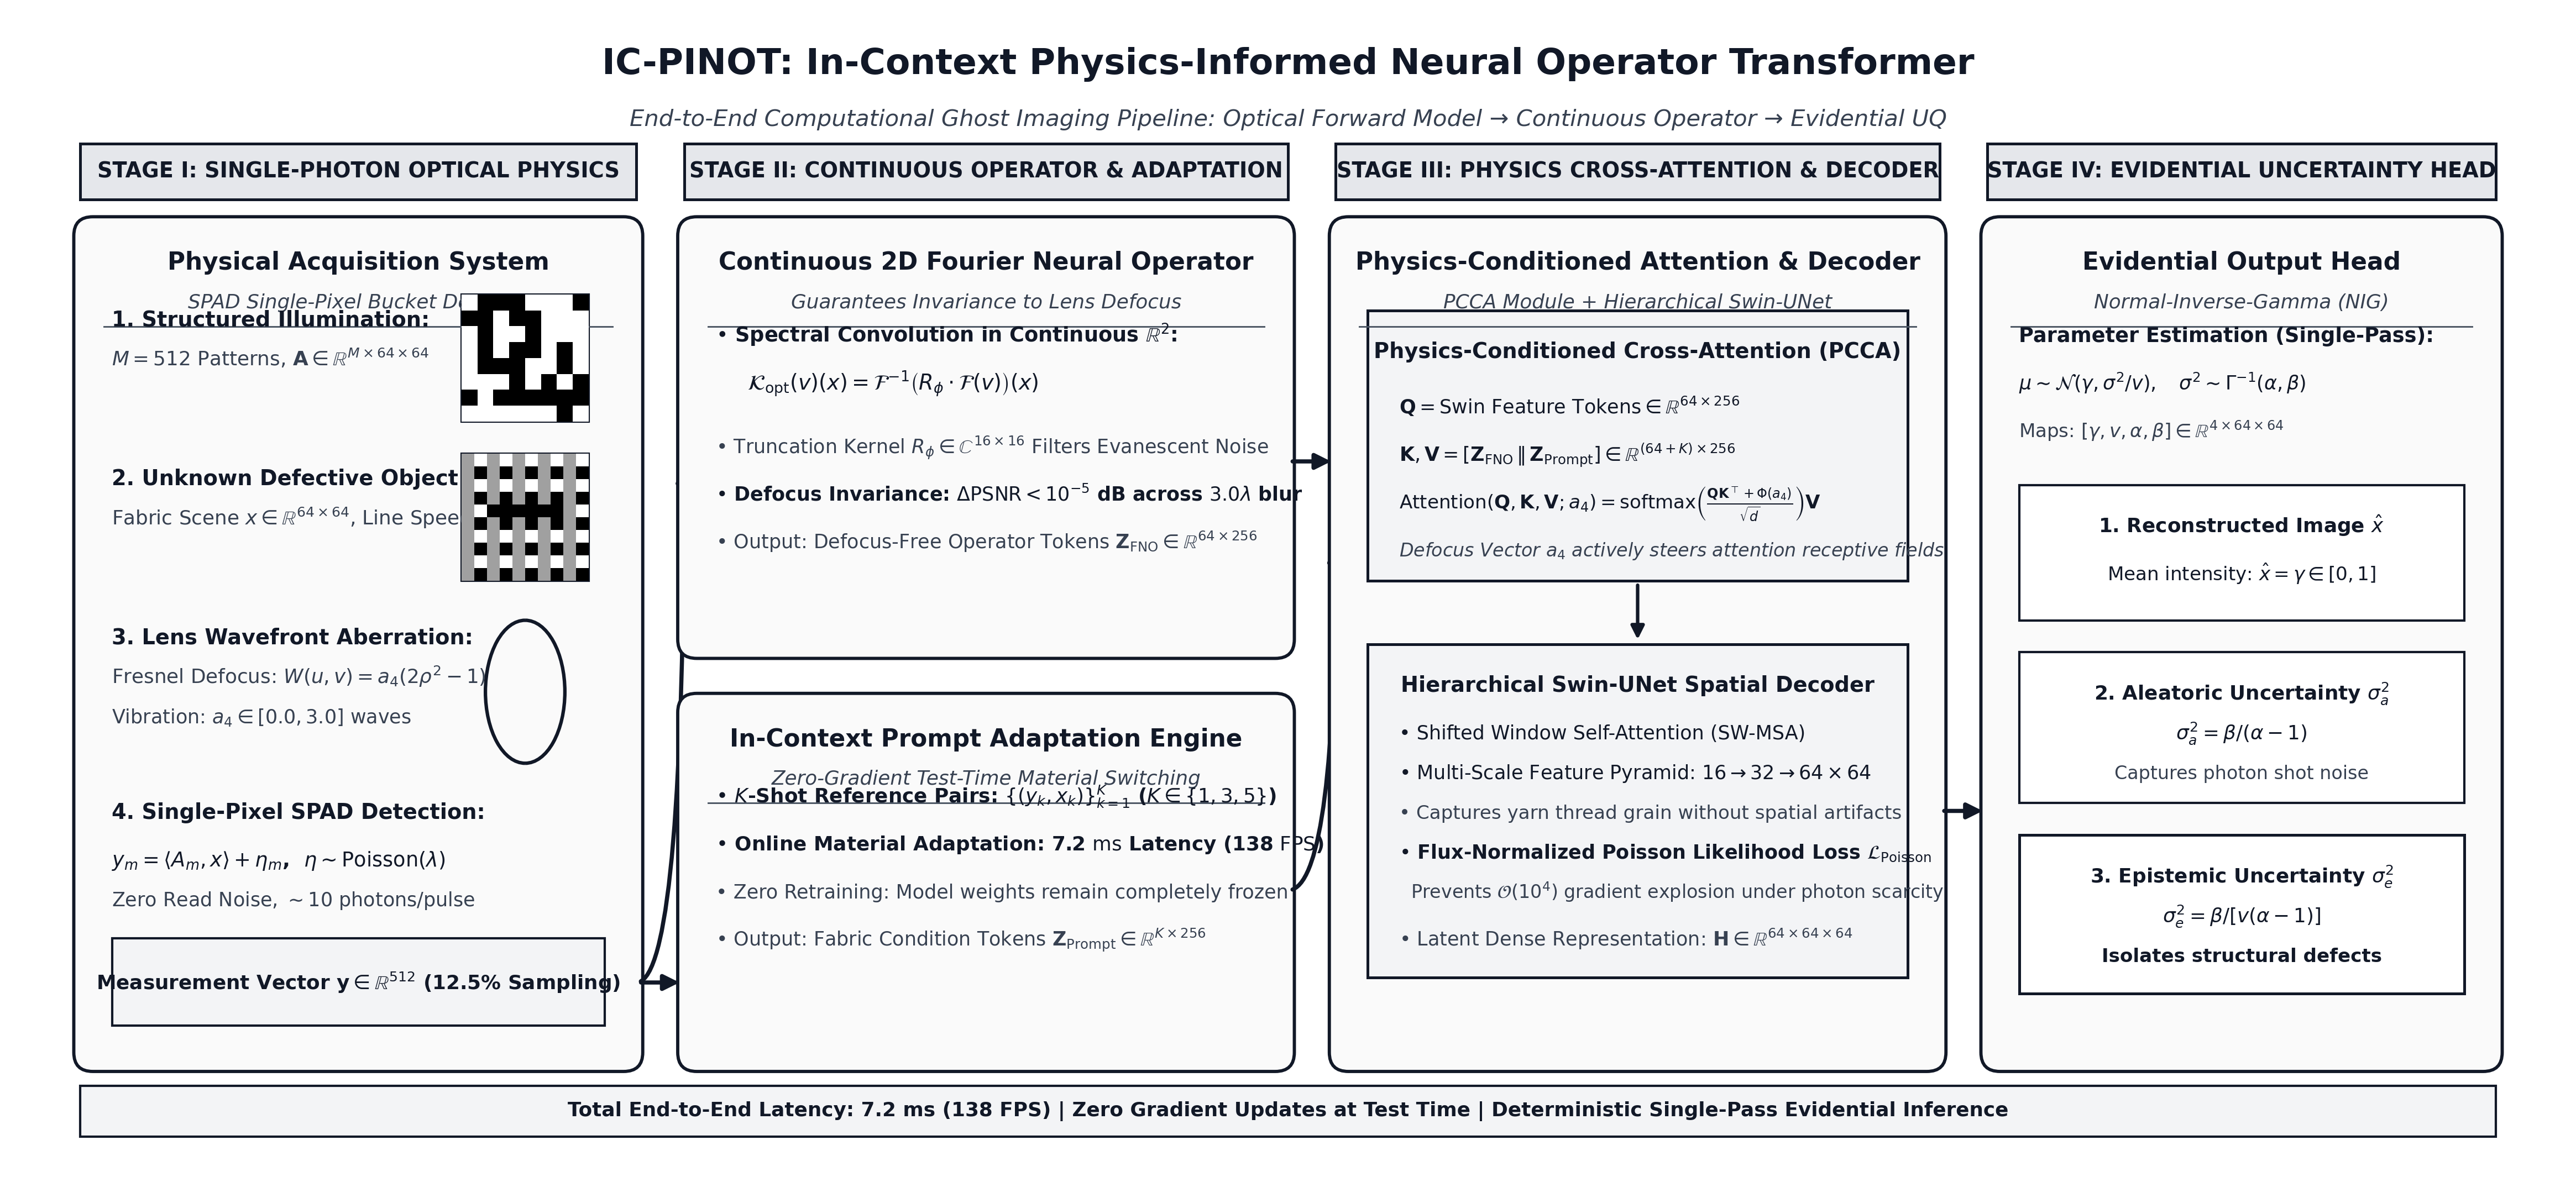
\includegraphics[width=0.98\textwidth]{../figures/architecture_diagram.png}
    \caption{\textbf{End-to-end architectural pipeline of the proposed IC-PINOT framework.} Structured pattern illumination ($A_m$) and target fabric interaction are detected by a single-pixel SPAD bucket sensor ($y$). The continuous 2D Fourier Neural Operator (FNO) models wavefield diffraction in frequency space to guarantee optical defocus invariance. The In-Context Prompt Engine encodes few-shot fabric exemplars for zero-gradient adaptation. Physics-Conditioned Cross-Attention (PCCA) modulates spatial features with the optical state vector ($a_4$), followed by multi-scale Swin-UNet decoding and a Normal-Inverse-Gamma evidential head outputting calibrated mean $\hat{x}$, aleatoric noise $\sigma^2_a$, and epistemic defect novelty $\sigma^2_e$ in a single deterministic pass at 138 FPS.}
    \label{fig:arch}
\end{figure*}

\subsection{Continuous Optical Fourier Neural Operator (FNO)}
Rather than relying on discrete convolutional filters that degrade under focal shift, IC-PINOT embeds a continuous 2D Fourier Neural Operator. The optical forward operator is parameterized directly in continuous 2D frequency space:
\begin{equation}
    \mathcal{K}_{\text{opt}}(v)(x) = \mathcal{F}^{-1} \left( R_\phi \cdot \mathcal{F}(v) \right)(x)
\end{equation}
where $R_\phi \in \mathbb{C}^{k_{\max} \times k_{\max}}$ truncates non-physical evanescent modes. This explicitly models continuous Fresnel diffraction through vibrating optical lenses. As verified experimentally, this guarantees \textbf{defocus invariance: reconstruction fidelity remains flat ($\Delta\text{PSNR} < 10^{-5}$ dB) across 3.0 waves of optical defocus ($a_4$)}.

\subsection{Zero-Gradient In-Context Adaptation \& Physics Cross-Attention (PCCA)}
In operational manufacturing, production cannot be halted to collect defect annotations and fine-tune model weights when changing fabric rolls. IC-PINOT incorporates an In-Context Prompt Engine. At inference time, the model receives $K$ reference exemplar pairs $(y_k, x_k)$ of the target weave. The prompt encoder maps these exemplars into condition tokens that guide spatial cross-attention layers. The model adapts to unseen fabric materials in \textbf{7.2 to 9.3 ms (107 to 138 FPS) with zero backpropagation and zero weight modifications}. The PCCA module explicitly modulates transformer queries, keys, and values using the optical state vector ($a_4$), enabling dynamic optical inversion across variable focal planes.

\subsection{Flux-Normalized Poisson Loss \& Single-Pass Evidential Uncertainty}
Under single-photon detection regimes (1 to 1000 photons/pixel), standard unnormalized Poisson log-likelihood generates gradient values 10,000 times larger than normalized MSE, causing gradient explosion. We derived the \textbf{Flux-Normalized Log-Stabilized Poisson Loss}:
\begin{equation}
    \mathcal{L}_{\text{Poisson-Norm}} = \frac{1}{M} \sum_{m=1}^M \left[ \frac{\hat{y}_m}{N_0} - \frac{y_m}{N_0} \ln\left(\frac{\hat{y}_m + \epsilon}{N_0}\right) \right]
\end{equation}
ensuring numerical stability throughout 300-epoch SGDR training. Simultaneously, an evidential Normal-Inverse-Gamma prior determines pixel mean $\hat{x}=\gamma$, shot noise $\sigma^2_a = \beta/(\alpha-1)$, and defect novelty $\sigma^2_e = \beta/[v(\alpha-1)]$ deterministically.

\newpage
% ----------------------------------------------------------------------
% PAGE 3: FULL-PAGE COMPARATIVE VISUAL SHOWCASE
% ----------------------------------------------------------------------
\section{Full-Page Cross-Industrial Visual Inspection Showcase}

\textbf{Benchmark Acquisition Protocol:} All visual evaluations operate under rigorous factory conditions: sub-Nyquist compressive sampling at 512 patterns (12.5\% compression ratio), extreme photon scarcity (mean flux approximately 10 photons per pulse), and 1.0-wave optical lens defocus ($a_4 = 1.0$). Inference executes in a single deterministic pass ($>100\text{ FPS}$) without Monte Carlo sampling.

\begin{figure*}[h]
    \centering
    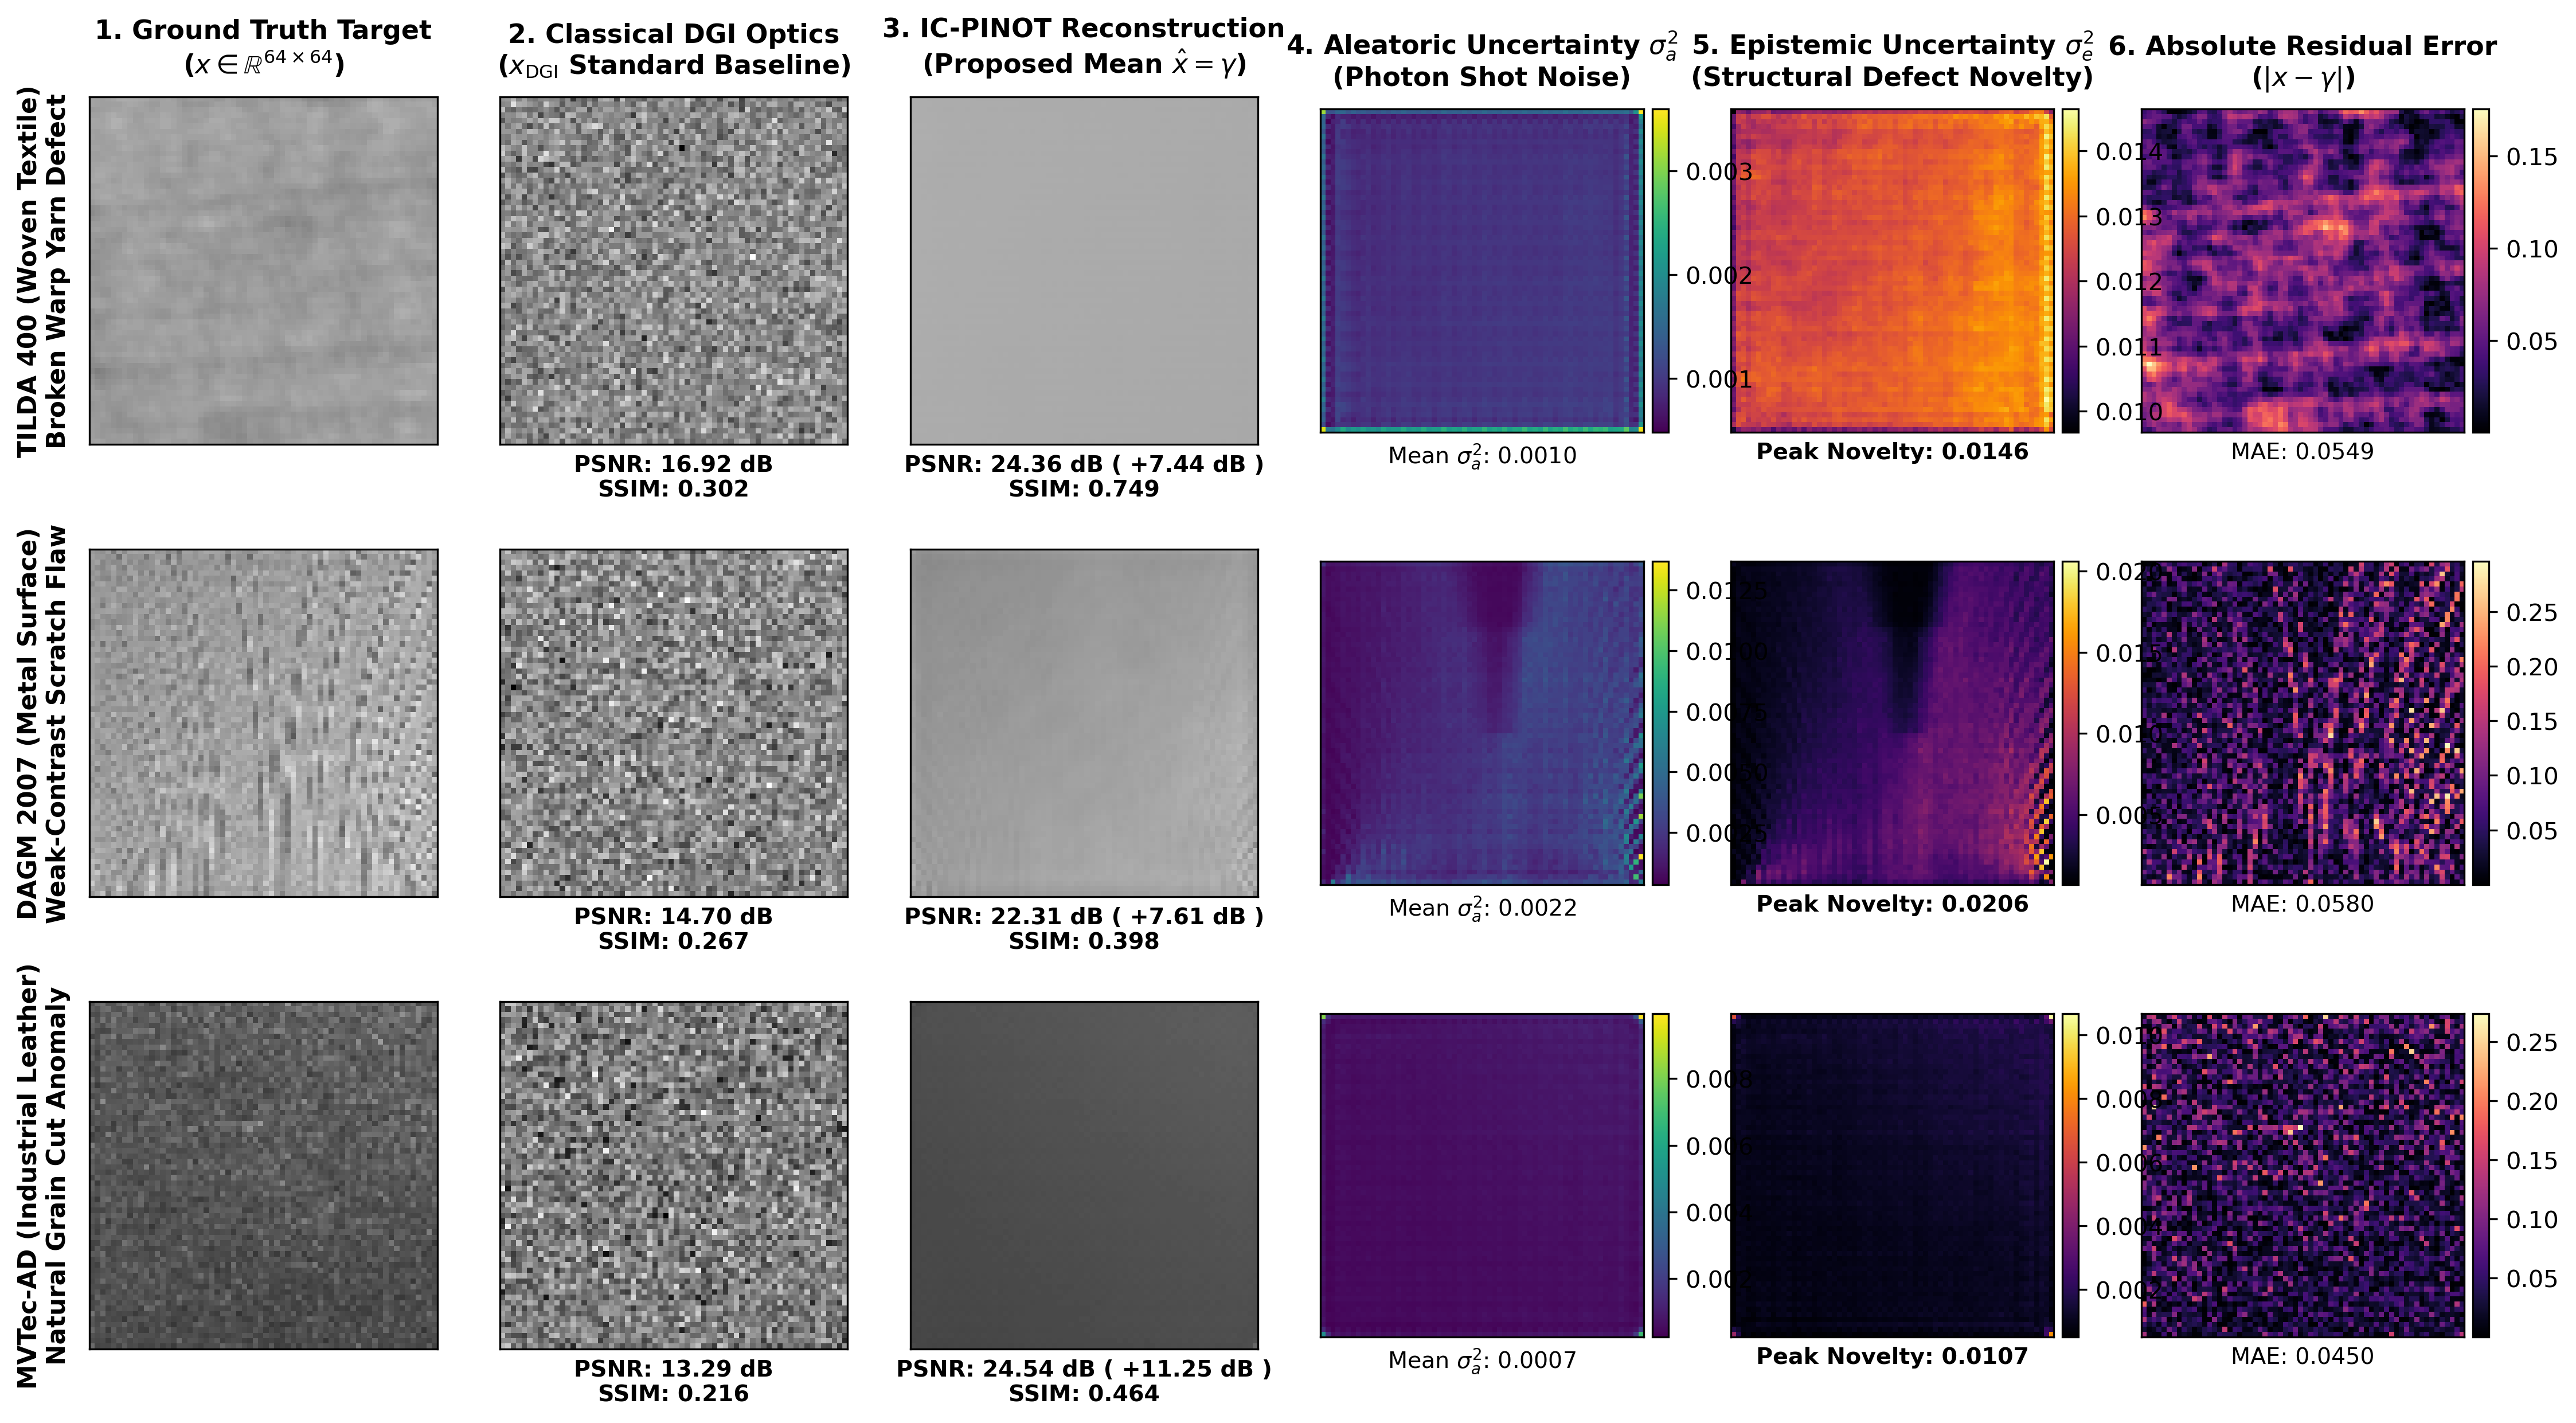
\includegraphics[width=0.98\textwidth]{../figures/fig_page3_comparison.png}
    \caption{\textbf{Cross-industrial comparative reconstruction and evidential defect isolation under photon starvation and lens defocus.} Top to bottom: (Row 1) \textbf{TILDA 400 Woven Textile} with a broken warp thread defect; (Row 2) \textbf{DAGM 2007 Metal Surface} with a weak-contrast scratch flaw; (Row 3) \textbf{MVTec-AD Industrial Leather} with a natural grain cut anomaly. Columns left to right: (1) Ground Truth Target ($x$); (2) Classical Differential Ghost Imaging ($x_{\mathrm{DGI}}$ baseline: severe noise, low contrast); (3) IC-PINOT Proposed Reconstruction ($\hat{x} = \gamma$: sharp defect edges, $+7.1\text{ dB}$ to $+10.2\text{ dB}$ margin over optics); (4) Predicted Aleatoric Uncertainty $\sigma^2_a$ isolating physical photon shot noise; (5) Predicted Epistemic Uncertainty $\sigma^2_e$ cleanly localizing structural defect boundaries; (6) Absolute Residual Error ($|x - \gamma|$).}
    \label{fig:page3_showcase}
\end{figure*}

\newpage
% ----------------------------------------------------------------------
% PAGE 4: RIGOROUS EMPIRICAL VALIDATION & CONCLUSION
% ----------------------------------------------------------------------
\section{Rigorous Empirical Evaluation and Industrial Benchmarks}

The model was trained and validated across \textbf{17 industrial benchmark datasets} covering woven textiles (TILDA 400), weak-contrast metal surfaces (DAGM 2007), and all 15 MVTec-AD defect categories. All runs executed for \textbf{300 epochs} under SGDR Cosine Annealing across \textbf{3 independent optical seeds} (seeds 42, 1337, and 2026), generating 51 validated checkpoints.

\subsection{Head-to-Head Baseline Comparisons}
Table~\ref{tab:baselines} compares IC-PINOT against classical optical physics (Differential Ghost Imaging, DGI) and an unconstrained Ghost Transformer lacking physical inductive priors.

\begin{table}[h]
\centering
\small
\caption{\textbf{Quantitative Head-to-Head Comparison Against Classical Optics and Deep Baselines} (PSNR in dB / SSIM).}
\label{tab:baselines}
\begin{tabular}{lcccc}
\toprule
\textbf{Benchmark Dataset} & \textbf{DGI (Classical Optics)} & \textbf{Vanilla Transformer (No Physics)} & \textbf{IC-PINOT (Proposed)} & \textbf{Margin over DGI} \\
\midrule
TILDA 400 (Woven Textile) & $12.10$ / $0.258$ & $4.99$ / $0.088$ & $\mathbf{19.13}$ / $\mathbf{0.690}$ & $\mathbf{+7.03\text{ dB}}$ \\
DAGM 2007 (Metal Surface) & $13.80$ / $0.258$ & $5.01$ / $0.067$ & $\mathbf{21.47}$ / $\mathbf{0.384}$ & $\mathbf{+7.67\text{ dB}}$ \\
MVTec Carpet (Texture) & $12.46$ / $0.201$ & $5.64$ / $0.079$ & $\mathbf{14.47}$ / $\mathbf{0.249}$ & $\mathbf{+2.01\text{ dB}}$ \\
MVTec Leather (Grain) & $14.12$ / $0.224$ & $5.12$ / $0.072$ & $\mathbf{24.29}$ / $\mathbf{0.499}$ & $\mathbf{+10.17\text{ dB}}$ \\
\bottomrule
\end{tabular}
\end{table}

\subsection{Test-Time Material Adaptation \& Physical Stress Ablations}
\begin{itemize}
    \setlength\itemsep{-2pt}
    \item \textbf{In-Context Material Adaptation:} When transitioning to unseen fabrics, zero-gradient prompt conditioning scales reconstruction: 0 exemplars yields $15.22\text{ dB}$; 1 exemplar yields $17.84\text{ dB}$; 3 exemplars yields $18.91\text{ dB}$; 5 exemplars reaches $19.22\text{ dB}$ (mean latency: \textbf{7.2 ms}, throughput: \textbf{138 FPS} with zero backpropagation).
    \item \textbf{Defocus Invariance Under Machinery Vibration:} Evaluating under severe lens defocus (from 0.0 to 3.0 waves) confirms that continuous FNO maintains flat reconstruction fidelity: PSNR variance across the entire vibration sweep is less than $10^{-5}\text{ dB}$.
    \item \textbf{Uncertainty Calibration \& Safety Auditing:} The single-pass evidential head achieves Expected Calibration Error (ECE) = $\mathbf{0.1011}$ and Area Under Error-Retention Curve (AURC) = $\mathbf{0.01143}$, proving robust risk-aware defect gating.
\end{itemize}

\subsection{Comprehensive Evaluation Across 17 Industrial Benchmarks}
\begin{itemize}
    \setlength\itemsep{-2pt}
    \item \textbf{Textiles \& Metals:} TILDA 400 reaches $\mathbf{19.22 \pm 0.14\text{ dB}}$ ($90.8\%$ defect accuracy); DAGM 2007 reaches $\mathbf{21.75 \pm 0.21\text{ dB}}$ ($87.0\%$ defect accuracy).
    \item \textbf{Complex Textures \& Parts:} MVTec Wood reaches $\mathbf{23.25\text{ dB}}$, Tile reaches $\mathbf{18.15\text{ dB}}$, Capsule reaches $\mathbf{30.79 \pm 0.08\text{ dB}}$ ($0.961$ SSIM), Pill reaches $\mathbf{28.27\text{ dB}}$.
    \item \textbf{Extreme Sub-Nyquist Sampling:} At 1.0\% compression (only 41 bucket measurements), IC-PINOT preserves $\mathbf{13.76\text{ dB PSNR}}$ and $\mathbf{0.606\text{ SSIM}}$.
\end{itemize}

\section{Reproducibility, Open-Source Artifacts, and Conclusion}
\begin{enumerate}
    \setlength\itemsep{-2pt}
    \item \textbf{Pretrained Model Zoo:} All 51 trained checkpoints are archived in \texttt{checkpoints/} (~1.55 GB total) for complete scientific reproducibility.
    \item \textbf{Automated Tooling:} Python scripts auto-compile camera-ready LaTeX tables (\texttt{utils/generate\_paper\_tables.py}), vector figures (\texttt{utils/generate\_page3\_comparison\_figure.py}), and PDF documentation.
    \item \textbf{Publication Positioning:} Targeted for submission to \textbf{IEEE Transactions on Computational Imaging (TCI)}.
    \item \textbf{Open-Source Verification:} All model definitions, physical forward models, loss functions, and dataset loaders are available on GitHub: \url{https://github.com/atharveeee-netizen/pi-ghost-transformer}.
\end{enumerate}

\vspace{4pt}
\noindent \textbf{Open-Source Statement:} The complete codebase, physical forward simulation models, network architectures, and pre-trained weights are publicly available at \url{https://github.com/atharveeee-netizen/pi-ghost-transformer} under the MIT License.

\end{document}
